\documentclass[11pt,a4paper]{article}
\usepackage[left=2.5cm,top=2cm,right=2.5cm,nofoot]{geometry}
\usepackage{geometry}
\usepackage{amsmath}
\usepackage{amssymb}
\usepackage{txfonts}
\usepackage{microtype}
\usepackage{epsfig}
\usepackage{graphicx}
\usepackage{moreverb}
\usepackage{hyperref}
\usepackage{listings}
\usepackage{xcolor}
\usepackage{textcomp}
\usepackage{makecell}
\usepackage{wasysym}
\definecolor{listinggray}{gray}{0.98}
\definecolor{lbcolor}{rgb}{0.98,0.98,0.98}
\lstset{
	backgroundcolor=\color{lbcolor},
	tabsize=4,
	rulecolor=,
	language=matlab,
    basicstyle=\scriptsize\ttfamily,
    upquote=true,
    aboveskip={1.5\baselineskip},
    columns=fixed,
    showstringspaces=false,
    extendedchars=true,
    breaklines=true,
    prebreak = \raisebox{0ex}[0ex][0ex]{\ensuremath{\hookleftarrow}},
    frame=single,
    showtabs=false,
    showspaces=false,
    showstringspaces=false,
    identifierstyle=\ttfamily,
    keywordstyle=\color[rgb]{0,0,1},
    commentstyle=\color[rgb]{0.133,0.545,0.133},
    stringstyle=\color[rgb]{0.627,0.126,0.941},
}

\usepackage{tikz}
\usepackage{pgfplots} 
\usepackage{pgfgantt}
\usepackage{pdflscape}
\usepackage{subcaption}
\usepackage{adjustbox}
\usepackage{siunitx}
\pgfplotsset{compat=newest} 
\pgfplotsset{plot coordinates/math parser=false}
\usepackage{pdfpages}
\usepackage{placeins}
\usepackage{wrapfig}





\newlength\fwidth
\newlength\fheight
\pagestyle{myheadings}

\pgfplotsset{every axis/.append style={
        scaled y ticks = false, 
        scaled x ticks = false, 
        y tick label style={/pgf/number format/.cd, fixed, fixed zerofill,
                            int detect,1000 sep={\;},precision=3},
        x tick label style={/pgf/number format/.cd, fixed, fixed zerofill,
                            int detect, 1000 sep={},precision=3}
    }
}

\usepackage{eso-pic}
\usepackage{ifthen}

\usepackage[nottoc]{tocbibind}
\usepackage[backend=biber,style=numeric,sorting=none]{biblatex}
\addbibresource{bibben.bib}

\usepackage{float}
\usepackage{subcaption}
\usepackage{gensymb}
\usepackage{siunitx}
\usepackage{enumitem}

\title{Project 2b: Bayesian Optimization}
\author{
  Kevin Andersson\\
  \texttt{kevinan@student.chalmers.se}
  \and
   Eric Lindgren\\
  \texttt{ericlin@chalmers.se}
}

\markright{Kevin Andersson and Eric Lindgren, Group 7}

\begin{document}

\maketitle

\pagenumbering{gobble}% Remove page numbers (and reset to 1)
% \newpage
\pagenumbering{arabic}% Arabic page numbers (and reset to 1)
\setcounter{page}{1}
\section{Introduction and Background}

One system of interest in materials science is one where an adsorbed atom, an adatom, is located on top of a crystal surface \cite{wiki_adatom}. The position of the adatom on the surface affects the total potential energy of the system, and thus the position of the adatom $(x,y)$ parametrizes a potential energy surface (PES) $E(x,y)$ for the system. However, there are two main problems when simulating such a system. First, finding the position of the adatom that results in the lowest energy is difficult since the PES often has multiple local minima \cite{project_pm}. Secondly, the system potential energy is often obtained using Density Functional Theory (DFT), and hence it may be computaionally intractable to perform many evaluations of the potential energy.

Both of these challenges will be tackled in this report using Gaussian Processes (GP). The first problem will be approached using Bayesian Optimization, and for the second problem we will train a general purpose model for the PES using only $\sim 100$ potential energy samples. This general purpose model can then be used instead of DFT to study various properties of the adatom \cite{project_pm}. We will specifically apply the general purpose model to predict the potential energy along a transition path for the adatom between two points on the crystal surface, and compare this to the ground-truth transition path as obtained from the PES.

The system of interest in this report is an Au-surface with an Au adatom. Note that this system will be simulated using atomistic simulations through the Python package \texttt{ASE} \cite{ASE}, and hence the ground-truth PES is being computed through MD simulations rather than DFT. However, this report still exemplifies the usefulness of Bayesian Optimization and GP-models for functions that are difficult to evaluate.

\section{Methodology}

In this section we present our methodology for analyzing and approximating the potential energy surface (PES) using Bayesian optimization for a Au surface with an Au atom placed on top. But before we go into detail on the Bayesian optimization, we first present the ground-truth PES that will be used as a basis for the optimization, as well as the results for trying to find the global minimum of the PES using naive local search which serves as a sort of baseline.


\begin{figure}[ht]
    \centering
    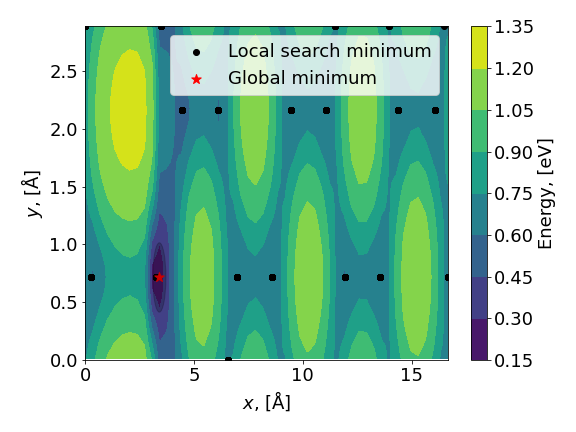
\includegraphics[width=0.7\textwidth]{figures/task12.png}
    \caption{Obtained potential energy surface (PES) together with the global minimum (red star) and the minima as obtained through a naive local search with 500 individual walkers (black dots). }
    \label{fig:pes}
\end{figure}

The Au system was simulated using \texttt{ASE}, a Python package for atomistic simulations \cite{ASE}, with the surface being given. In order to obtain the PES $E(x,y)$, the surface atom was introduced at different coordinates $(x,y,z)$ with $z$ being set so that the surface atom was placed some distance above the surface, after which the system was relaxed using BFGS as implemented in \texttt{ASE}. The obtained PES is given in figure \ref{fig:pes}, with the global minimum being marked with a red star. Note that there are many local minima in the PES; a quick visual inspection yields that there are at least 12 local minima. We thus expect that conducting a local search to find the global minimum starting from random positions $(x,y)$ should succeed with a probability around $p \approx 1/12 \approx 8\%$. We performed such a search using 500 walkers with random starting positions, which were then minimized using the \texttt{minimize} function from the Python package \texttt{Scipy} setup to use the gradient-based L-BFGS-B method \cite{scipy_min}. The optimum found by each walker are given in figure \ref{fig:pes} as black dots. The local search resulted in 10\% of the walkers converging to the global minimum, which is slightly higher than our expectation, but still highlights the difficulty of performing optimization in complex energy landscapes using (naive) local gradient descent-based algorithms. Thus it is motivated to use methods such as Bayesian optimization, which we will focus on throughout the rest of this report. 

\subsection[Task 1]{Task 1-2: Analyzing the PES and local search}
\label{sec:method_task12}

\subsection[Task 1]{Task 3: Bayesian Optimization}
\label{sec:method_task3}
In this task we want to perform a Bayesian optimization algorithm to find the global minimum, but also sample the PES as few times as possible. In general sample the PES our any other multidimensional function can bee very expensive and time consuming, as in this case performing a DFT calculation. This Bayesian optimization algorithms is based on Gaussian processes (GP) which can be viewed as an infinite dimensional Gaussian distribution where each point in the $(x,y)$-plane is a dimension. The function modelled  by the GP (the PES) is then uniquely determined via the GPs covariance function. So bye conditioning the GP on some data we get a distribution for the PES everywhere in the $(x,y)$-plane. In this task we used the GPy packege to handle all implementation of the GP so we only need to choose how we determine the covariance function. The covariance function is modeled by a kernel and we will use the radial basis function (RBF) kernel which looks like 
\begin{equation*}
    k(x, x') = \sigma^2 \text{exp}(-\frac{1}{2l^2}||x - x'||_{L2}^2),
\end{equation*}
where $\sigma^2$ and $l$ is two parameters known as the kernel variance and the kernel length scale. The kernel variance is in a way the amplitude of the covariance and thus describe how large the variations are in the PES. So from figure \ref{fig:pes} we see that the PES has extremums  at 7 eV and 8 eV so the standard deviation maybe lie around 0.3 and the variance then 0.09. So we choosed to set a gamma distributed prior for $\sigma^2 \sim \mathcal{G}(1,0.1)$. The length scale determines how far between the points need to be to not be regarded as correlated, or in other words over how large regions are the PES roughly constant or slowly varying. So from figure \ref{fig:pes} we can see that maximum extends over roughly 0.5 Å. We thus set a prior for the length scale to be a gamma distribution $\mathcal{G}(2,0.5)$ which has mean 0.5 Å.
\\

We have now described the basic of a GP and specify a kernel and priors for our parameters and can thus make prediction $\mu(x,y)$ with standard deviation uncertainty $\delta(x,y)$ over the hole primitive cell. So we now need to define where we want to sample a new point, from our prediction. To decide this we define the acquisition function
\begin{equation*}
    A(x,y) = -\mu(x,y) + \beta \delta(x,y),
\end{equation*}
where beta is a hyper parameter we must choose. By finding the the point where the acquisition function as a maximum we sample point where the PES is low and where the GP is uncertain, and the hyperparameter thus balance if we think exploitation or exploration is more important. To summarise the algorithm then consist of first evaluate the PES at 5 random points, training the GP model and do a prediction of the PES. From the prediction we then evaluate the PES again for a point obtained by maximizing the acquisition function and then train a new GP with the new data point. This is then repeated until one is satisfied with the sampling.  
\\

So we now have the complete Bayesian optimisation algorithm and the next part is to decide a good value of the hyper parameter $\beta$. To do this we performed the optimization for many values of $\beta \in (1,5)$ and then evaluated the performance by looking at the convergence. So keeping in mind that we generally want to find the global minimum and evaluate the PES as few times as possible we define convergence to be when the GP finds the global minimum. With this definition we can decide the hyper parameter by choosing the $\beta$ that resulted in least amount of samples. 





















\subsection[Task 4]{Task 4: Transition path barriers}
\label{sec:method_task4}

In this task, we study GPs as a way of emulating the full PES. Using GPs to emulate the PES yields a fast model which can be used to compute various properties related to the adatom \cite{project_pm}. In this case, we will specifically focus on using the GP model to analyze a transitional path barrier. 

Here we will study the specific transition path through the PES that connects the point $(11,2.1)$ with the global minimum. This could thus be viewed as a having the adatom transition from a position on the Au surface that yields a local minimum in the system energy, to a configuration that minimizes the total system energy. An arbitrary path between the points $(x_1,y_1)$ and $(x_2,y_2)$ can be parameterized by a parameter $\lambda$ that varies between $0\rightarrow1$ as

\begin{equation}
    (x,y) = \left(x_1, y_1 \right ) + \lambda \left(x_2-x_1, y_2-y_1 \right).
\end{equation}
Thus by evaluating the GP mean of the obtained model for points $(x,y)$ for various $\lambda$, we obtained the sought transition path as a function of $\lambda$. The uncertainty in the GP prediction along the path was estimated by evaluating the GP variance along the same points $(x,y)$. These results could then be compared to the Bayesian Optimization GP from Task 3 and the ground-truth PES evaluated along the same path. 

In order to obtain a GP model that emulates the ground-truth PES to a high degree, we require a slightly different sampling behaviour as compared to the previous task in section \ref{sec:method_task3}. The key quantity to minimize is the overall uncertainty of the GP over the $\{x,y\}$-domain, and thus we want to sample points where the GP uncertainty is the largest. Thus, the LCB acquisition function in equation \eqref{eq:acquisition_function} was modified by letting $\beta \rightarrow \infty$ \cite{project_pm}. The GP model was then trained by sampling points according to this modified acquisition function, and the convergence of the model was monitored by computing the RMSE (root-mean-squared-error) of the GP mean as compared to the ground truth PES. The same priors, grid size for the acquisition function and number of starting initial data points as in task 3, section \ref{sec:method_task3}, where used.

\section{Results and discussion}

In this section we present our result for cutoff and feature selection in a cluster expansion, as well as for the Bayesian cluster expansion and its comparison to OLS in predicting ground state candidates. 

\subsection[Task 1]{Task 3: Bayesian Optimization}
\label{sec:results_task3}
To evaluate the model for different values of the hyper parameter $\beta$ figure \ref{fig:task3_iter} is presented. In the figure we see how many iterations it took before the optimization algorithm found the global minimum. From the it is clear that the algorithm does not converge for all values of beta, in particular algorithms with to small $\beta$ never finds the global minimum. However we also see from the figure that to large $\beta$ demands more iteration before convergence. Both of these features seems reasonable; for small $\beta$ the algorithm is more likely to keep sampling a local minimum instead of exploring more of the space. This then resulting in sensitivity for the location of the starting point and we end up in the same situation we got for the naive search on task 2. For large $\beta$ we are on the other hand more inclined to explore new parts of the space even if we already samples near the global minimum. This may lead to the sinareo where we found the global minimum but we have not sampled it fine enough to determine it exact location, this scenario could also be very dependent on the convergence condition; how close to the global minimum do you need to sample to say you found it. So from the figure we seem to have a optimal value for the hyper parameter somwhere around $\beta = $???, for which the algorithm finds the global minimum the fastest. However this result is only valid for when we send in this particular set of initial data, for another set of data which is closer to the global minimum the algorithms with low $\beta$ might find it much faster. But also if the global minimum would have been farther away from the initial data maybe algorithms with $\beta$ higher then ??? also would have had trouble finding it. So to decrease this uncertainty and be more confident in the choice of beta one should do this sweep over the hyper parameter many times where different initial data is used and then present the average number of iterations.

To further extend on this analysis the choice of convergence criteria is a bit arbitrary and can highlight different aspect of the algorithm. An alternative definition of convergence could for example be when the algorithms samples the same point (to some tolerance) two or more times in a row. This convergence criterion is probably also very sensitive to the initial data, but if that uncertainty is eliminated (as described above) algorithms with lower $\beta$ should always converge faster. The problem is that it does not always converge to the global minimum so one here also need to consider how many times (different initial data) the algorithms finds the global minimum for each value of $\beta$ and then balance the two curves of the convergence and efficiency of finding the global minimum. To use this convergence condition may be more reasonable since we in a general situation do not know the global minimum and then needs some other condition when to stop sampling. In the other case the thing we really are interasted in is to find the global minimum with as few evaluations of the PES as possible which the convergence condition we used highlights. However both of these methods to decide $\beta$ and especially the condition we used probably  generalize poorly to other functions since it could be very sensitive to the form of the function.

\begin{figure}[H]
    \centering
    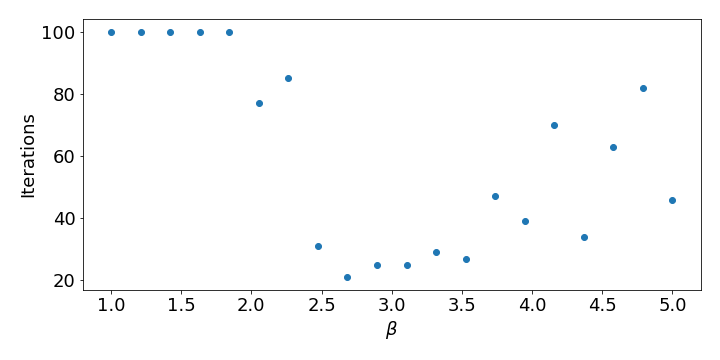
\includegraphics[width = 0.8\textwidth]{figures/task3_iter.png}
    \caption{Caption}
    \label{fig:task3_iter}
\end{figure}

\begin{figure}[H]
    \centering
    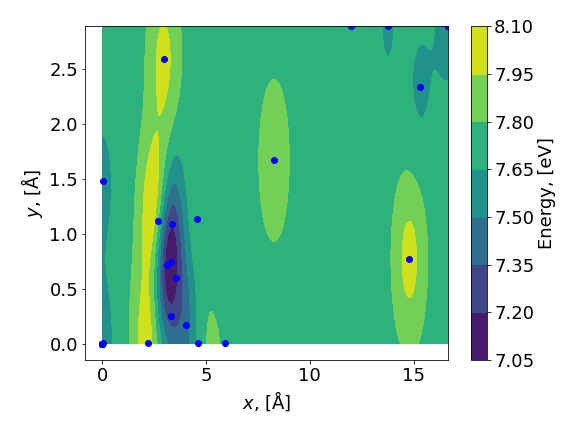
\includegraphics[width = 0.8\textwidth]{figures/task3_mean.png}
    \caption{Caption}
    \label{fig:my_label}
\end{figure}

\begin{figure}[H]
    \centering
    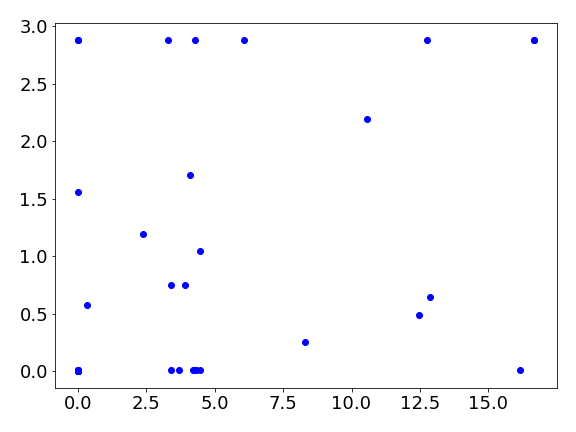
\includegraphics[width = 0.8\textwidth]{figures/task3_var.png}
    \caption{Caption}
    \label{fig:my_label}
\end{figure}

\begin{figure}[H]
    \centering
    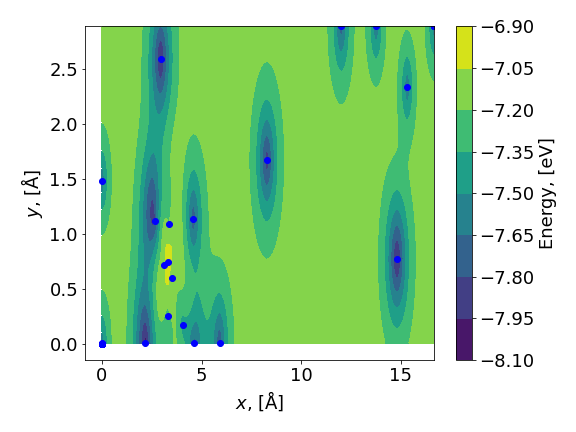
\includegraphics[width = 0.8\textwidth]{figures/task3_acq.png}
    \caption{Caption}
    \label{fig:my_label}
\end{figure}

So once we had decided on a good value for $\beta = $??
? we rerun the algorithm and the result is presented in figure \ref{fig:task3_pred}. In the figure we see prediction of the GP for the PES together with the predicted uncertainty and the acquisition function. This all for the last step in the algorithms, i.e when we converged. From the mean plot we can clearly see that it has found the global minimum and capture the features of the the PES close to the minimum. For other regions however the GP does not capture the PES, which is good since we only are interested in finding the Global minimum. From the figure we also see a heat map for the standard deviation uncertainty over the primitive cell. We can see that the uncertainty varies a bit over the cell and is generally much lower near the samples, which is expected. From the figure we also see the acquisition function which as expected balance the search between searching the found minimum and the uncertain areas. We can also see that the acquisition function that is large in a big portion of the area..... 


One interesting observation that can be made from the figure is that many of the sampled point lay along the edges of the primitive cell. This feature was generally observed when performing the optimization and was even more prominent when we had more samples. We conclude that this most be because the GP becomes much more uncertain in its prediction near the edges. This is very reasonable since the edge break the symmetry of where nearby sampled points are located from which we can use in the inference. This effectively leads to at this points the GP is almost doing an extrapolation instead of an interpolation. However we now that the primitive cell is periodic so in a sens we have sampled points outside the boundary condition, this information is unfortunately not used in the GP. Having said that this can be built in the GP by using a periodic kernel instead. We made some attempts with the Standard periodic kernel but had some trouble with instability of the method. But when it worked the sampling was distributed much better over the primitive cell and we avoided sampling the edge over and over again. Ulltimatly this leads to the need of fewer samples and we strongly believe that the best way to sample this PES is to use the knowledge of periodicity in the GP by encoding it in the kernel. 


\begin{figure}[H]
    \centering
    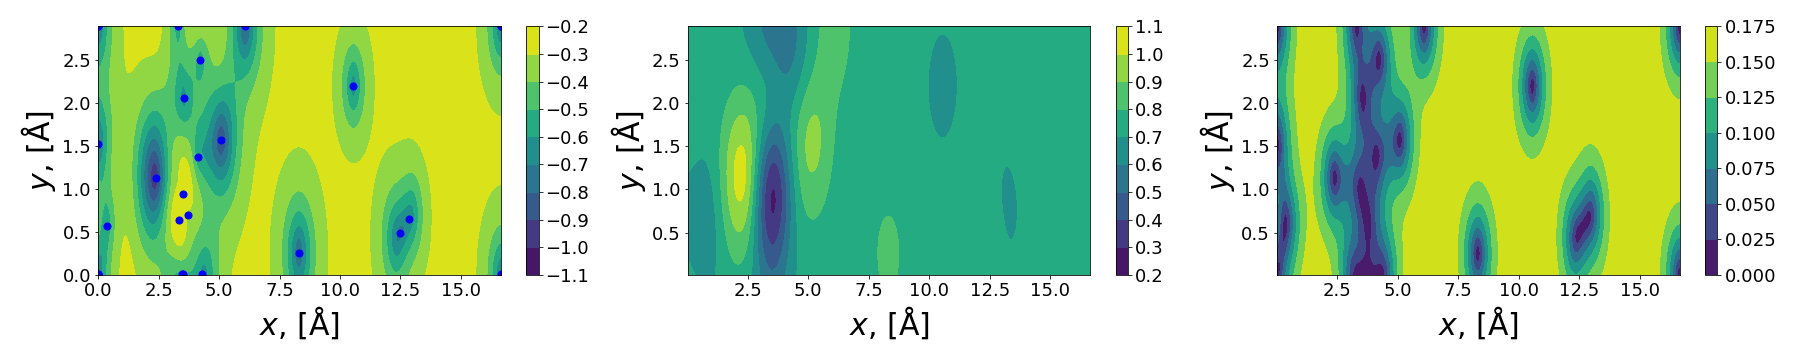
\includegraphics[width = 1\textwidth]{figures/task3_pred.png}
    \caption{Caption}
    \label{fig:task3_pred}
\end{figure}

\subsection[Task 4]{Task 4: Transition path barriers}
\label{sec:results_task4}

We finally turn to the results for the use of a general GP as a proxy for the PES, and how it can be used to predict a transition path for the adatom on the Au surface. The RMSE as monitored during training of the GP is given in figure \ref{fig:task4_rmse}. The RMSE is computed as the root-mean-squared error between the GP mean and the ground-truth PES, and is given as a function of the number of training samples as acquired by the modified acquisition function. We note that the training RMSE features some plateaus and fluctuations. The plateaus could correspond to local minimum in the GP optimization landscape, and the fluctuations could be due to the model not having fully converged and thus not being ''robust''. However, after around 120 samples the RMSE starts to decrease monotonously, and seems to flatten out at around 150 samples at a low training RMSE of $\SI{0.04}{eV}$. We thus conclude that around 150 samples are required to reach a general GP that represents the ground-truth PES well. 

\begin{figure}[ht]
    \centering
    \begin{subfigure}{.46\textwidth}
          \centering
          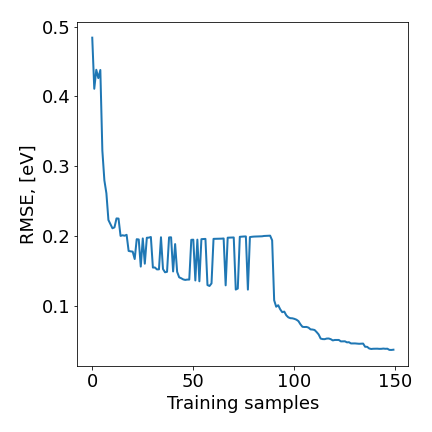
\includegraphics[width=0.95\textwidth]{figures/task4_train.png}
          \caption{Training RMSE for general GP}
          \label{fig:task4_rmse}
    \end{subfigure}%
    \begin{subfigure}{.46\textwidth}
          \centering
          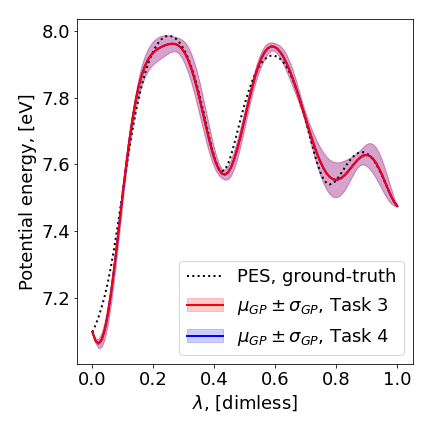
\includegraphics[width=0.95\textwidth]{figures/task4_path.png}
          \caption{Predicted and ground-truth transition path}
    \label{fig:task4_transition}
    \end{subfigure}
    \caption{}
    \label{fig:task4}
\end{figure}

The potential energy transition path for the adatom transitioning between two points on the Au-surface is given in figure \ref{fig:task4_transition}. The mean predicted path from the general GP (referred to as Task 4), $\mu_{GP}$ is given as the blue filled line, with a one standard deviation error band obtained from the GP variance, $\sqrt{\sigma^2_{GP}}$, represented by the blue shadowed area. The mean predicted path for the Bayesian optimization GP (Task 3) is given as the red dashed line, with the one standard deviation error band given by the red shadowed area. Finally, the ground-truth transition path as obtained from the PES is given as the dotted black line. We observe that both the mean and the one-standard deviation error bands for both the Bayesian optimization GP and the general GP overlap almost perfectly. Furthermore, both GPs seems to model the the ground-truth PES fairly well, with it being mostly covered by the one-standard deviation error band. However, both GP models undershoots the ground-truth close to the global minimum, i.e. for $\lambda\approx 0$, except for at the minimum point $\lambda = 0$. These results indicates two things. First,  that Bayesian optimization using fairly few data points, $\sim 20$, performs as well as the general GP trained using $\sim 100$ data points for this transition path. Thus, our results indicate that one can decrease the number of points one needs to sample by optimizing the LCB acquisition function and setting an optimal $\beta$ for a balance between exploration and exploitation of the PES. The general GP can hence be viewed as more of a ``brute-force'' approach. Secondly, that the GP models reproduce the PES fairly well motivates that Gaussian processes in general could be effectively used as a proxy model for the PES to compute properties of the system with reasonable accuracy, in situations where the ground-truth PES is difficult to sample and one thus has access to a limited number of data points. However, there are some deviations for the GP models, especially around the global minimum ($\lambda\approx 0$), and hence the specific GP models studied in this report may not be perfectly suitable for applications which depend on a accurate modelling around the global minimum. It is possible that the use of other kernels which utilize more information of the system, such as the Standard periodic kernel discussed in the previous section, may be able to represent the area around the global minimum with higher accuracy.

% TODO Lägg till modell från task 3



\newpage
\printbibliography

\end{document}
